\documentclass[]{article}
\usepackage{lmodern}
\usepackage{amssymb,amsmath}
\usepackage{ifxetex,ifluatex}
\usepackage{fixltx2e} % provides \textsubscript
\ifnum 0\ifxetex 1\fi\ifluatex 1\fi=0 % if pdftex
  \usepackage[T1]{fontenc}
  \usepackage[utf8]{inputenc}
\else % if luatex or xelatex
  \ifxetex
    \usepackage{mathspec}
  \else
    \usepackage{fontspec}
  \fi
  \defaultfontfeatures{Ligatures=TeX,Scale=MatchLowercase}
\fi
% use upquote if available, for straight quotes in verbatim environments
\IfFileExists{upquote.sty}{\usepackage{upquote}}{}
% use microtype if available
\IfFileExists{microtype.sty}{%
\usepackage{microtype}
\UseMicrotypeSet[protrusion]{basicmath} % disable protrusion for tt fonts
}{}
\usepackage[unicode=true]{hyperref}
\hypersetup{
            pdfborder={0 0 0},
            breaklinks=true}
\urlstyle{same}  % don't use monospace font for urls
\usepackage{graphicx,grffile}
\makeatletter
\def\maxwidth{\ifdim\Gin@nat@width>\linewidth\linewidth\else\Gin@nat@width\fi}
\def\maxheight{\ifdim\Gin@nat@height>\textheight\textheight\else\Gin@nat@height\fi}
\makeatother
% Scale images if necessary, so that they will not overflow the page
% margins by default, and it is still possible to overwrite the defaults
% using explicit options in \includegraphics[width, height, ...]{}
\setkeys{Gin}{width=\maxwidth,height=\maxheight,keepaspectratio}
\IfFileExists{parskip.sty}{%
\usepackage{parskip}
}{% else
\setlength{\parindent}{0pt}
\setlength{\parskip}{6pt plus 2pt minus 1pt}
}
\setlength{\emergencystretch}{3em}  % prevent overfull lines
\providecommand{\tightlist}{%
  \setlength{\itemsep}{0pt}\setlength{\parskip}{0pt}}
\setcounter{secnumdepth}{0}
% Redefines (sub)paragraphs to behave more like sections
\ifx\paragraph\undefined\else
\let\oldparagraph\paragraph
\renewcommand{\paragraph}[1]{\oldparagraph{#1}\mbox{}}
\fi
\ifx\subparagraph\undefined\else
\let\oldsubparagraph\subparagraph
\renewcommand{\subparagraph}[1]{\oldsubparagraph{#1}\mbox{}}
\fi

% set default figure placement to htbp
\makeatletter
\def\fps@figure{htbp}
\makeatother


\date{}

\begin{document}

\textbf{\emph{SCHIZOFRENIA:}}

\textbf{\emph{STORIA:}}

\begin{itemize}
\item
  \textbf{\emph{KRAEPELIN (1850):}}
\end{itemize}

Primo concetto importante è che la schizofrenia non nasce con il nome di
schizofrenia, ma il primo nome che venne dato è di \textbf{Demenza
Precox} (significa letteralmente demenza precoce), cioè un quadro di
demenza, ovvero progressivo deterioramento della personalità, capace di
insorgere precocemente (età tra i 16 e 25 anni ) e dopo un decorso
progressivo portare ad uno stato di completa disgregazione.

Il concetto di demenza precox nasce a cavallo tra `800 e `900 in un
periodo caratterizzato per la psichiatria di un completo nichilismo
terapeutico(non esistevano psicofarmaci). I primi farmaci per i disturbi
psichici nascono attorno anni '50, prima c'erano i manicomi e i medici
non potevano fare altro che osservare 24h su 24 senza la possibilità di
modificare il decorso della malattia. Anche la terapia elettroconvulsiva
(elettroshock) nasce nei primi del '900.

Il termine demenza precox fu coniato da uno psichiatra tedesco di nome
\textbf{Emil Kraepelin} che è stato il fondatore della nosografia
psichiatrica, prima di lui erano già stati descritti segni e sintomi
psichiatrici, ma non era ancora stata data una coerenza nosografica.

Kraepelin fece un'operazione semplice: divise i pazienti in due gruppi
secondo un criterio longitudiale, cioè secondo il decorso della malattia
e indipendentemente dai sintomi:

\begin{itemize}
\item
  \emph{Il primo gruppo era caratterizzato da un deterioramento
  progressivo} e quindi da un quadro cronico della patologia (non
  andavano in contro a remissione e stavano in manicomio tutta la vita);
\item
  \emph{il secondo gruppo era caratterizzato da quei pazienti che
  inspiegabilmente andavano incontro a remissione} anche dopo quadri
  gravi cronici.
\end{itemize}

Il primo modello classificatorio delle malattie mentali gravi era quindi
\textbf{in base alla prognosi}: quelli che guarivano e quelli che non
guarivano.

\begin{itemize}
\item
  Quelli che non guarivano erano inclusi nell'ambito della
  \textbf{demenza precox} (corrisponde alla moderna schizofrenia)
\item
  gli altri invece venivano classificati nell'ambito delle
  \textbf{psicosi maniaco depressive} (che corrisponde essenzialmente al
  disturbo bipolare, anche se autori successivi hanno poi distinto le
  forme di depressione unipolare)
\end{itemize}

Si notò che quelli che avevano una prognosi migliore erano quelli che
presentavano più frequentemente sintomi affettivi o in senso depressivo
o in senso espansivo; notò anche che i pazienti con psicosi
maniaco-depressive avevano un decorso fasico, ovvero episodico, con
episodi gravi e poi dopo risoluzione (a differenza del primo gruppo che
non aveva fasi, ma andava incontro a destrutturazione progressiva).

Kraepelin incluse nella demenza precox quadri che erano già stati
precedentemente descritti come per esempio: la catatonia , ebefrenia,
visania atipica, tutte caratterizzate dall'esito infausto, dall'esordio
giovanile (in genere tra i 16 ed i 25 anni) e con un decorso più o meno
rapidamente progressivo che portava nell'arco di una decina d'anni ad
una condizione pressoché irreversibile.

\begin{quote}
Quindi riassumendo, il primo concetto importante è che Kraepelin fece
una distinzione e definì quella che poi venne definita schizofrenia in
base alla prognosi. L'unica possibilità di fare diagnosi, però, era il
tempo; il criterio di Krepelin era dunque un \emph{criterio
longitudinale}: non era possibile fare diagnosi al primo colloquio con
un paziente ma solo considerando l'evoluzione e il decorso clinico,
quindi la diagnosi di Dementia Precox veniva confermata quando si
riconosceva nel paziente l'evoluzione progressiva e l'esito infausto
(diagnosi a posteriori).
\end{quote}

Quando parlava di demenza si riferiva ad uno stato degenerativo
difficile da immaginare, perché non c'erano farmaci e il decorso era
diverso da ora (epoca in cui ci sono i farmaci).

\begin{itemize}
\item
  \textbf{\emph{BLEULER (1911):}}
\end{itemize}

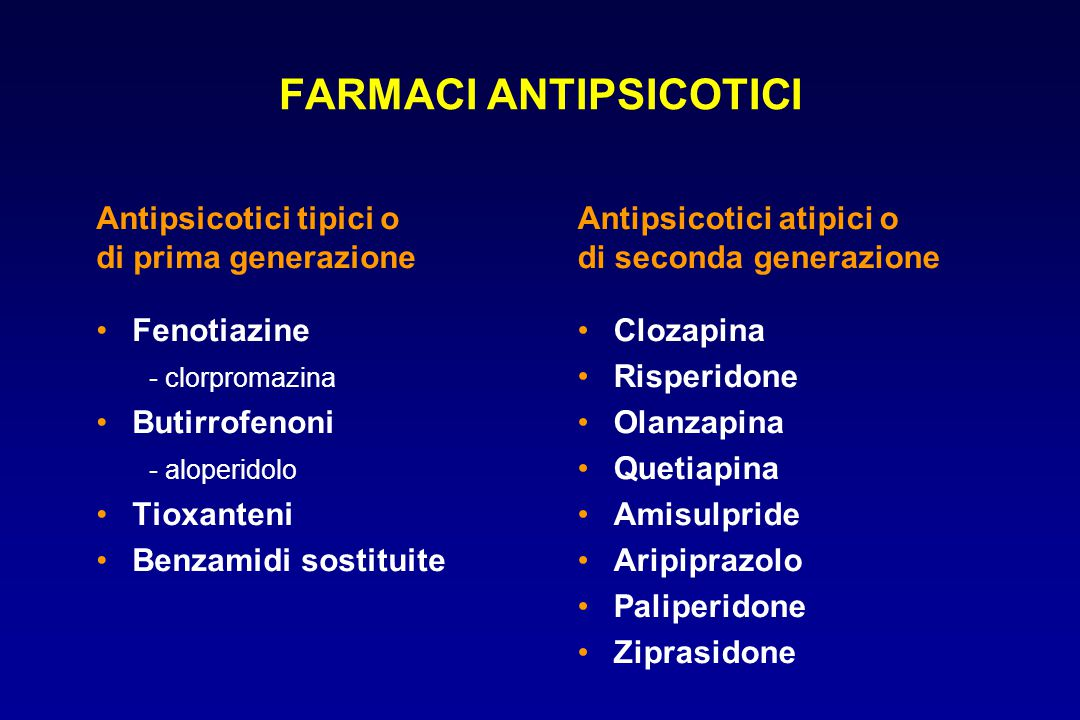
\includegraphics[width=4.00000in,height=3.55482in]{media/image1.jpeg}

\emph{\emph{Definizione:}}

Quindi il problema rimaneva di fare diagnosi: nel 1911 \textbf{Bleuler}
completò il concetto di \textbf{schizofrenia}, adottando non più un
criterio longitudinale, ma \emph{trasversale}: fare diagnosi a partire
dai sintomi.

Fu il primo a coniare il termine schizofrenia al posto di demenza
precox(che si rifà a concezione longitudinale invece che trasversale).

Schizofrenina, letteralmente ``\textbf{\emph{rottura della mente}}'',
proprio per introdurre un \emph{criterio trasversale} e non più
longitudinale, ovvero indipendente dal decorso. Per Bleuler, la
schizofrenia è un disturbo che si caratterizza per una
\textbf{\emph{scissione}}, una ``\textbf{spaltung}'' \emph{delle
funzioni psichiche}, cioè una \emph{perdita della coesione strutturale
della personalità ed una dissociazione delle funzioni psichiche} che
porta, indipendentemente dal decorso, ad una \emph{discordanza}, ad una
\emph{frattura}, una \emph{disarmonia tra le varie funzioni psichiche},
in particolare l'\textbf{affettività}, la \textbf{memoria} e la
\textbf{coscienza}: ovvero tutto ciò che coinvolge la vita psichica
dell'individuo viene scissa, diventa discordante. Se riusciamo a
cogliere nel paziente questa perdita di coesione della personalità,
possiamo ipotizzare diagnosi di schizofrenia senza aspettare del tempo.

Le varie funzioni psichiche sono discordanti.

\emph{\emph{Criteri:}}

Bleuler andò oltre e definì alcuni sintomi fondamentali per la diagnosi,
distinguendoli da quelli accessori (che potevano anche non esserci).

\textbf{SINTOMI FONDAMENTALI:}

\begin{itemize}
\item
  disturbi affettività: apatia più o meno grave
\item
  abulia: perdita della volontà
\item
  autismo schizofrenico (non autismo infantile)
\item
  ambivalenza
\item
  dissociazione ideica
\end{itemize}

Sintomi tutti in negativo.

\textbf{SINTOMI ACCESSORI:}

\textbf{●} disturbi percettivi

● deliri

● disturbi memoria e della personalità

●sintomi catatonici

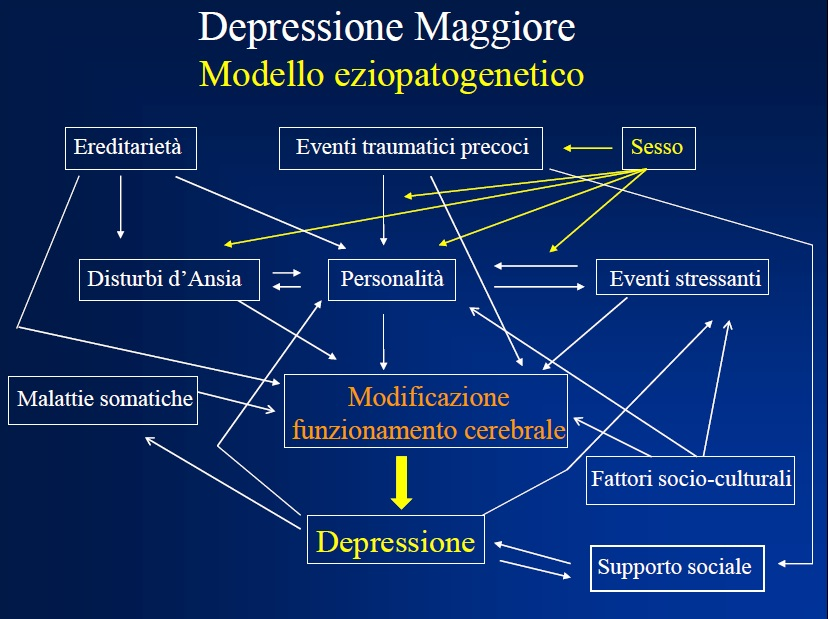
\includegraphics[width=5.02222in,height=3.97361in]{media/image2.jpeg}

\begin{quote}
Distinse anche i sintomi in un altro modo (che non ha a nulla a che fare
con la distinzione precedente)

\textbf{PRIMARI} = non generati da altri sintomi (disturbi associativi,
perturbazione umore di fondo)

\textbf{SECONDARI} = conseguenza di sintomi primari (autismo,
ambivalenza, deterioramento schizofrenico, deliri, sintomi catatonici)

Ad es autismo schizofrenico è sia sintomo fondamentale ma anche
secondario (a deliri e allucinazioni)
\end{quote}

Caratteristicamente lo schizofrenico è identificato come una persona
soggetta ad allucinazioni, deliri, catatonia. I sintomi fondamentali,
ovvero l'essenza della schizofrenia, non sono questi sintomi eclatanti:
anzi questi appartengono a molti quadri clinici diversi anche dalla
schizofrenia. La schizofrenia non è questo quadro.

Ad esempio:\emph{ragazzi che si chiudono in casa e a cui non importa più
di fare nulla, sono trascurati e l'eloquio comincia a disgregarsi
indipendentemente dai deliri e allucinazioni.}

Anzi i quadri più gravi sono quelli caratterizzati da questi sintomi
negativi.

\emph{\emph{Decorso:}}

I sistemi nosografici attuali ereditano i concetti storici. Importante
ricordare è che la \emph{schizofrenia ha un decorso cronico e non
fasico: una volta che inizia, tende ad avanzare.} Questo decorso cronico
porta sempre ad un meno rispetto a prima.

La schizofrenia, inoltre, può instaurarsi sia come
\textbf{\emph{processo}} che come \textbf{\emph{sviluppo}}:

\begin{itemize}
\item
  \emph{Come processo}: esordio acuto o iperacuto. l'entità morbosa si
  abbatte improvvisamente e senza preavviso sul soggetto, spezzando la
  continuità di significato della vita di quel paziente
\end{itemize}

\begin{quote}
Il paziente era in un modo e nell'arco di pochi giorni o mesi inizia a
presentare sintomi che lo portano a distaccarsi da quello che era
precedentemente.

Sintomi di solito positivi: deliri, allucinazioni. Talvolta può avvenire
a più tappe: fase acuta, parziale remissione, altra fase acuta e
progressione (prognosi più favorevole).
\end{quote}

\begin{itemize}
\item
  \emph{Come sviluppo}: non acuta ma subdola, graduale, meno eclatante.
\end{itemize}

\begin{quote}
Lento scivolamento a partire da tratti di personalità morbosi che erano
predisponenti alla malattia. Persone che da sempre erano introverse, con
difficoltà di relazione che, però, funzionavano: quindi personalità
predisposte, che nell'arco di mesi cominciano, ad esempio, a chiudersi
in casa o distaccarsi progressivamente. Di solito meno importanti
sintomi produttivi, ma sono in primo piano i sintomi negativi, con
completa destrutturazione personalità. Sono i casi più a rischio di non
essere individuati precocemente ( prognosi più sfavorevole). Più di
frequente essa esordisca a partire da una personalità premorbosa,
condizione nota come \textbf{schizoidia}, la quale non è quindi una
malattia, ma un tratto di personalità predisponente alla schizofrenia, e
la si ritrova:
\end{quote}

-nel \emph{DP schizotipico}

-nel \emph{DP schizoide}

Nella schizoidia è presente una personalità con una tendenza al
disadattamento progressivo che favorisce quindi la nascita della
schizofrenia.

La schizoidia si caratterizza per una peculiare disposizione e tendenza
a porre una distanza tra sé e l'ambiente, e la persona appare chiusa,
introversa, quasi fredda, non ricercando l'amicizia o il contatto con
gli altri; non sono timidi ma sono semplicemente disinteressati, poiché
presi da interessi personali inusuali, che non condividono con altri.

Altra caratteristica della schizoidia è un'\textbf{anomala}
\textbf{proporzione psicoestesica}, ovvero la compresenza di
\emph{iperestesia} (elevata sensibilità e suscettibilità alle critiche)
e \emph{anestesia affettiva} (indifferenza alla rete delle relazioni
sociali).

\begin{itemize}
\item
  \textbf{\emph{SCHNEIDER (1967):}}
\end{itemize}

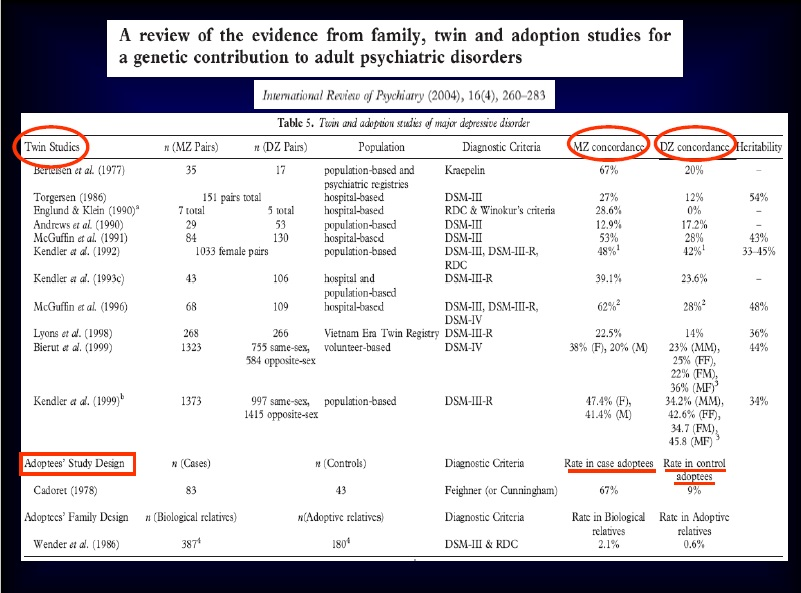
\includegraphics[width=4.80000in,height=3.92174in]{media/image3.jpeg}

Il tedesco \textbf{Schneider} aggiunge un ultimo tassello. Da una parte
la schizofrenia è un processo neurodegenerativo che rimane soprattutto
caratterizzato da sintomi negativi, ma Schneider dice una terza cosa:
spesso è difficile riconoscere questi sintomi fondamentali, che sono più
fini dei sintomi negativi, con il rischio di ritardare la diagnosi.

Lui identifica dei sintomi positivi che sono caratteristici della
schizofrenia (come deliri e allucinazioni) che hanno la caratteristica
fondamentale di un vissuto di PASSIVITA'.

Sono i \textbf{\emph{SINTOMI di PRIMO RANGO}}, altamente predittivi di
schizofrenia:

\begin{itemize}
\item
  \textbf{Allucinazioni uditive o pseudo allucinazioni: }
\end{itemize}

\begin{enumerate}
\def\labelenumi{\arabic{enumi}.}
\item
  \begin{quote}
  possono essere VOCI TELEOLOGICHE: danno consigli e possono essere
  banali e far compagnia al paziente continuamente;
  \end{quote}
\item
  \begin{quote}
  possono essere DIALOGANTI: dialogano tra loro, avendo come argomento
  il paziente, spesso ne parlano male
  \end{quote}
\item
  \begin{quote}
  possono essere IMPERATIVE: danno ordini a volte banali, oppure
  addirittura di uccidersi o uccidere. Sono voci difficili da gestire,
  con pazienti che spesso non riescono a farle passare e quindi eseguono
  gli ordini che queste voci impongono, anche se non coincidono con la
  loro reale volontà. Quindi interferiscono molto con la vita del
  paziente;
  \end{quote}
\item
  \begin{quote}
  possono essere voci COMMENTANTI gli atti del paziente;
  \end{quote}
\item
  \begin{quote}
  possono essere come ECO DEL PENSIERO: ovvero ripetono quello che il
  paziente pensa e lui ha paura che gli altri possano sentirle.
  \end{quote}
\end{enumerate}

\begin{quote}
\emph{Queste voci hanno in comune la perdita della barriera tra l'io
intimo e il mondo, c'è senso di permeabilità tra il paziente e il
mondo.}

n.b: Sono presenti anche in disturbi depressivi e maniacali ma nella
Schizofrenia sono di tipi particolari e interferiscono con la vita del
pz.
\end{quote}

Altro sintomo di primo rango di Schneider:

\begin{itemize}
\item
  \textbf{Passività di pensiero}: paziente non più padrone del suo
  pensiero, imposto da altri.
\end{itemize}

\begin{enumerate}
\def\labelenumi{\arabic{enumi}.}
\item
  \begin{quote}
  Paziente distaccato da propri pensieri, fino a quando non diventa più
  suo pensiero, ma è il pensiero di un altro inserito nella sua testa.
  Come se fosse costretto così a pensare il pensiero di un altro, questa
  è l'INSERZIONE DEL PENSIERO;
  \end{quote}
\item
  \begin{quote}
  Oppure il FURTO DEL PENSIERO: il paziente pensa e il pensiero gli
  viene rubato da un altri. Questi vissuti espongono a deliri definiti
  DI SPIEGAZIONE dove il paziente cerca di darsi delle spiegazioni (ad
  esempio tramite sistemi satellitari, onde elettromagnetiche, ovvero
  spiegazioni deliranti);
  \end{quote}
\item
  \begin{quote}
  Anche fenomeni di LETTURA del pensiero, il pensiero del paziente è
  letto da altri spesso tramite macchinari, attraverso cose fisiche;
  \end{quote}
\item
  \begin{quote}
  DIFFUSIONE del pensiero: i pensieri dal paziente diffondono e si
  trasmettono agli altri.
  \end{quote}
\end{enumerate}

Tutto ciò si manifesta quindi spesso sotto forma di deliri, altre volte
i sintomi di primo rango si manifestano sotto forma allucinatoria di
vario tipo (ad esempio allucinazioni visive di diffusione del pensiero).

\begin{itemize}
\item
  \textbf{Passività somatica}: estraneità del proprio corpo (ad esempio
  altri che tramite mezzi ordinano o muovono parti del corpo senza
  volerlo). Il paziente riferisce di non essere lui a voler fare un
  movimento, ma è costretto, come una marionetta, e lo stesso vale anche
  per le altre funzioni biologiche, come la minzione.
\end{itemize}

Bisogna distinguere 2 momenti di gravità differente:

\begin{itemize}
\item
  perdita del senso di proprietà: ad esempio il braccio non è più il suo
  ma è stato sostituito (più grave)
\item
  perdita del senso di agenzia: ad esempio non è lui che muove braccio
  ma sono gli alieni ma il braccio è sempre del paziente.
\end{itemize}

Caso clinico: \emph{il prof fa l'esempio di un suo paziente che riferiva
non essere padrone della sua minzione perché la decisione di mingere gli
veniva imposta da un vecchietto appollaiato sulla sua prostata, quindi
passività somatica associata a delirio di interpretazione.}

Altri sintomi di primo rango secondo Schneider sono poi:

\begin{itemize}
\item
  \textbf{Passività di volontà e affettività}: volontà e sentimenti
  affettivi comandati o voluti da altri.
\item
  \textbf{Percezione delirante} (rara): poggia su un substrato di
  PASSIVITA' DI PERCEZIONE. La percezione delirante è una percezione
  corretta, ma a questa viene attribuita un significato abnorme ( caso
  clinico:\emph{paziente entra in una stanza vede una sedia e da lì
  capisce l'imminente venuta di Cristo sulla terra}). E' una passività
  di percezione perché il paziente è investito dal significato.
\end{itemize}

\begin{quote}
Diverse sono le interpretazioni deliranti (molto più frequente, non solo
nella schizofrenia ) che non sono sintomi di primo rango (caso clinico:
\emph{paziente vede semaforo rosso e dice che è rosso sangue e allora
significa che lo vogliono uccidere, il paziente attivamente attribuisce
significato al percetto)}. Nella percezione delirante non c'è questa
attività, ma è tutta passività, la modalità è rivelatoria, non di
conferma.
\end{quote}

I sintomi di primo rango hanno una modalità molto fisica, il paziente
sente fisicamente le cose per esempio i pensieri di altri che entrano in
lui li sente entrare, come se bruciasse la pelle.

Abbiamo una spazializzazione del pensiero: li sentono fisicamente
(\emph{ad esempio pensieri che sentono dietro l'orecchio}). Questo si
manifesta non solo per la passività di pensiero ma per tutti i livelli
di passività, anche per la passività somatica (ad esempio:
\emph{paziente che sente omino che sta sulla sua prostata che gli dice
quando deve andare in bagno}).

In tedesco questi disturbi di passività si definiscono
\emph{``\textbf{\emph{gemacht}}= participio passato di fare'': il
pensiero è fatto da altri} e tutto è vissuto in termini spazializzati,
fisici.

C'è un altro termine che corrisponde al ``gemacht'', il corrispettivo
dell'ambiente: ``\emph{\textbf{\emph{gestelt}}} = collocato, messo lì''.
Si manifesta molto nelle fasi iniziali. Tutto quello che il paziente
vede è messo lì apposta, come se fosse tutta una trama di una
sceneggiatura, scritta apposta per il paziente (ad esempio:
\emph{qualcuno ha messo un telecomando qui apposta per me per dirmi
qualcosa}); tutto ruota attorno al paziente.

Per la diagnosi attualmente devono essere presenti più sintomi di primo
rango di Schneider ma ancora più importante del numero è la pervasività
dei sintomi, cioè la loro incidenza nella vita psichica del pz.

\begin{quote}
Poi abbiamo i \textbf{\emph{SINTOMI DI SECONDO RANGO}} : sebbene siano
importanti non consentono la diagnosi di schizofrenia, e sono
rappresentati da:
\end{quote}

\begin{itemize}
\item
  \emph{intuizioni deliranti},
\item
  \emph{disturbi psico-sociali},
\item
  \emph{disturbi depressivo-euforici}
\item
  \emph{ottusità affettiva}.
\end{itemize}

\begin{quote}
Quindi \emph{riassumendo} la Schizofrenia è:
\end{quote}

\begin{itemize}
\item
  per \textbf{Krepelin}, una condizione a \emph{evoluzione verso la
  demenza}, indipendentemente dai sintomi.
\item
  per \textbf{Breuler}, una condizione caratterizzata dalla
  \emph{frattura dello psichismo}, indipendentemente dal decorso.
\item
  per \textbf{Schneider}, una condizione caratterizzata dal
  \emph{vissuto di passività.}
\end{itemize}

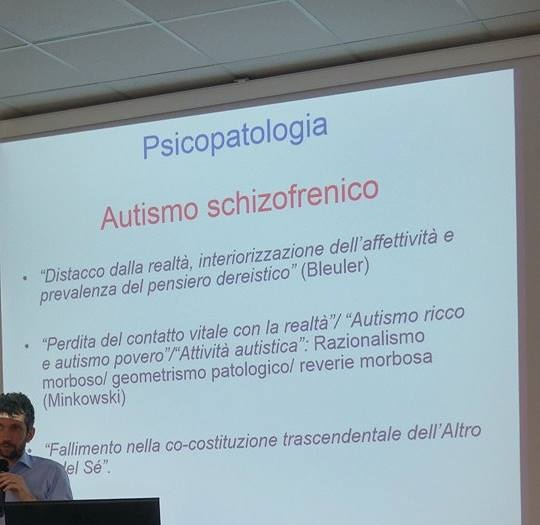
\includegraphics[width=3.85217in,height=3.22352in]{media/image4.jpeg}

\textbf{\emph{MANIFESTAZIONI CLINICHE DELLA SCHIZOFRENIA}}:

\textbf{\emph{AUTISMO SCHIZOFRENICO:}}

\begin{itemize}
\item
  \textbf{\emph{BLEULER:}}
\end{itemize}

Inserito da Bleuler nel 1911 tra i sintomi fondamentali.

Definizione classica:

\begin{itemize}
\item
  \emph{distacco dalla realtà,}
\item
  \emph{interiorizzazione dell'affettività} (si intende che
  l'affettività è introiettata verso l'interno, verso le proprie
  fantasie e interessi strampalati e non verso l'esterno o verso gli
  altri.
\item
  \emph{prevalenza di un pensiero dereistico} (che non tiene conto della
  realtà).
\end{itemize}

Bleuler con autismo intendeva un sintomo fondamentale della
schizofrenia, ma secondario, non primario, che corrispondeva al
progressivo distacco dalla realtà: ovvero il paziente non è più
interessato alle cose del mondo, della realtà e si chiude nel suo mondo
delirante, fantastico. Questo distacco si evince da un pensiero
destrutturato, da una \emph{perdita del senso comune} (common sense)
quindi la perdita di ciò che per noi è pre-riflessivo (non ci dobbiamo
pensare) e che ci permette di vivere in mezzo agli altri, tanto che i
pazienti si comportano un po' come degli alieni, non sanno più come
parlare o interagire con gli altri e non riescono nemmeno a
comprenderli.

\begin{itemize}
\item
  \textbf{\emph{MINKOWSKI:}}
\end{itemize}

Il concetto di autismo fu approfondito poi da un altro autore, Eugène
\textbf{Minkowski} (1927), che lo fece diventare il cardine della
schizofrenia.

Definisce l'autismo schizorfrenico come una \textbf{\emph{condizione di
perdita del contatto vitale con la realtà o una perdita dell'evidenza
naturale}}, cioè il paziente perde quel qualcosa che normalmente non era
consapevole di possedere, ma che gli consentiva di mantenersi attaccato
alla realtà. Ovvero quello che il paziente perde è quel qualcosa a cui
noi non pensiamo perché è riflessivo: quel qualcosa che serve per
interagire con gli altri, per fare le cose che sappiamo dalla nascita e
che il paziente va a perdere nella schizofrenia.

Minkowski divide l'autismo in:

\begin{itemize}
\item
  AUTISMO RICCO: è quando questo distacco dalla realtà è accompagnato da
  una ricca produttività delirante, allucinatoria.
\end{itemize}

\begin{quote}
Ad es un pz chiuso nella sua stanza vive mondi fantasmagorici (esempio
di un pz che ogni giorno andava su Orione per accoppiarsi con una
principessa aliena)
\end{quote}

\begin{itemize}
\item
  AUTISMO POVERO: distacco accompagnato dal nulla, i pazienti stanno in
  casa senza fare nulla, guardano il soffitto (molto più grave della
  forma ricca).
\end{itemize}

Secondo Minkowski, questa condizione può essere presente anche nelle
\textbf{\emph{personalità pre-morbose}}, dove assume il nome di
\textbf{attività autistica} e comprende essenzialmente 3 forme:

\begin{enumerate}
\def\labelenumi{\arabic{enumi}.}
\item
  RAZIONALISMO MORBOSO: il significato comune delle cose viene perduto,
  il paziente cerca di ricodificare la realtà in modo
  iper-razionalistico (ad esempio: \emph{padre che regala alla figlia
  malata di tumore una bara}). C'è un completo distacco dall'evidenza
  naturale del normale vivere comune.
\item
  GEOMETRISMO PATOLOGICO: (ad esempio: \emph{paziente che, prima di
  esordire, diceva di non riuscire a capire il perché il sabato sera si
  dovesse uscire con gli amici; gli era talmente inspiegabile da
  convincersi che i suoi amici con la macchina descrivessero dei
  triangoli, di cui lui doveva calcolare l'area}). Senso geometrico
  della realtà.
\item
  REVERIE (fantasticherie morbose): i pazienti si chiudono nel loro
  mondo e non vivono. Si costruiscono una realtà di fantasticherie
  simili a quelle dei bambini, non sono dei deliri (ad esempio:
  \emph{una paziente, vissuta in casa tutta la vita in condizioni
  pessime, si era presentata alla visita, raccontando di essere la
  fidanzata di Lapo Elkann, di essere una modella. Il tutto con la
  consapevolezza di non aver davvero compiuto i fatti dei suoi racconti,
  era solo una fantasia}).
\end{enumerate}

\begin{itemize}
\item
  \textbf{\emph{BISWANGER:}}
\end{itemize}

\begin{quote}
Dopo Minkowski un altro autore (\textbf{Biswanger}) definì altre 3
caratteristiche dell'autismo schizofrenico, \textbf{le 3 forme
dell'esistenza mancata:}
\end{quote}

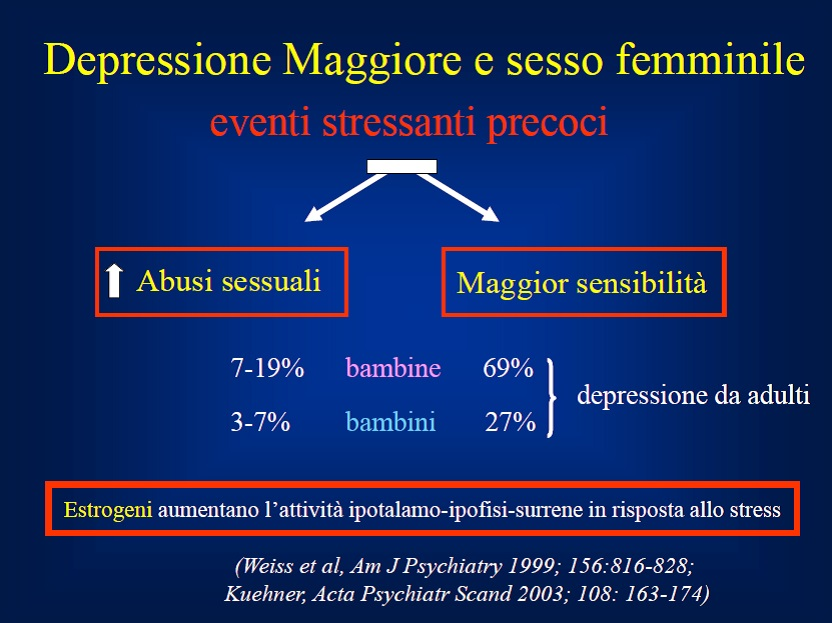
\includegraphics[width=3.31806in,height=2.15625in]{media/image5.jpeg}

\begin{enumerate}
\def\labelenumi{\arabic{enumi}.}
\item
  ESALTAZIONE FISSATA: pazienti in cui la perdita di contatto con la
  realtà si manifesta perché si fissano su una cosa che fa capire quanto
  il paziente sia distaccato. ( ad esempio: \emph{paziente che si era
  fissato sull'amicizia per un suo amico, viveva per questa amicizia,
  non sono deliri}; oppu oppure ad esempio: \emph{paziente che viveva
  solo per capire il meccanismo dell'orgasmo femminile, si documentava
  tantissimo e scriveva e lo spiegava in modo schizofrenico,
  meccanicistico}).
\item
  STRAMBERIA: caratteristica dell' andare di traverso rispetto a quello
  che il senso comune (ad esempio: \emph{il paziente che regala la bara
  alla figlia}; oppure: \emph{andare in giro con il piumino ad agosto};
  \emph{paziente che dorme durante la messa}).
\item
  MANIERISMO (molto frequente nella schizofrenia): paziente imita in
  modo goffo come ci si dovrebbe comportare con gli altri (ad
  esempio\emph{: paziente che, quando vedeva il dottore, lo salutava in
  modo esagerato ogni volta, anche a distanza di pochi minuti}). Alcune
  forme di schizofrenia si caratterizzano primariamente con questo
  comportamento.
\end{enumerate}

\textbf{\emph{DIMENSIONI DELLA SCHIZOFRENIA:}}\\
Attualmente, nei moderni sistemi nosografici, la schizofrenia viene
considerata come una sindrome che si caratterizza per la presenza di 3
dimensioni sintomatologiche:

\begin{enumerate}
\def\labelenumi{\arabic{enumi}.}
\item
  \textbf{\emph{DIMENSIONE NEGATIVA:}}
\end{enumerate}

I sintomi negativi coincido con i sintomi fondamentali di
\emph{Bleuler}, ad esclusione dei disturbi di associazione delle idee
che rientrano nella dimensione di disorganizzazione.

I sintomi negativi sono l'elemento nucleare della schizofrenia perché
tendono a persistere, sono refrattari alla terapia farmacologica; sono
la dimensione che maggiormente impatta sull'esito, sul funzionamento
globale del soggetto. comprende le cosiddette ``\emph{4 A di Bleuler}'',
ovvero \textbf{apatia} 8mancanza di sensazioni), \textbf{abulia}
(mancanza di volontà), \textbf{anedonia} (mancanza di piacere) e
\textbf{alogia} (povertà di pensiero), da cui deriva il \textbf{ritiro
sociale}.

Diversamente dei sintomi positivi, quelli negativi, così chiamati
proprio per indicare la mancanza di capacità di interazione sociale,
\emph{non rispondono alla terapia farmacologica e tendono a permanere
nel tempo}.

I sintomi negativi si distinguono in \textbf{due gruppi}: primari e
secondari.

\begin{itemize}
\item
  I \textbf{sintomi secondari} sono secondari ad altro: secondari a
  terapie con farmaci neurolettici di prima generazione, secondari
  all'istituzionalizzazione (processo cronico di sottostimolazione
  ambientale) oppure secondari a sintomi positivi, ad esempio: un
  paziente delira, è convinto che ci sia un complotto contro di lui, che
  qualcuno stia cercando di ammazzarlo, di conseguenza si chiude in
  casa. I sintomi secondari possono essere corretti correggendo la causa
  che sta alla base.
\item
  I \textbf{sintomi primari}, che sono i più interessanti, tendono ad
  essere acquistabili nel tempo e sono refrattari alla terapia.
\end{itemize}

\emph{Caso clinico}: \emph{A tale proposito si riporta l'esempio di un
paziente (35 anni) affetto da schizofrenia il cui quadro è
caratterizzato prevalentemente da sintomi negativi, quadro grave: il
paziente a gennaio riceve un invito a pranzo dalla sorella (unica
persona con cui il paziente intrattiene relazioni sociali, una persona
molto accudente, carina, persona di fiducia) per Ferragosto (da notare
gennaio-agosto intercorrono sei mesi tra l'invito e il pranzo). Il
paziente è molto angosciato per l'invito nonostante il pranzo sia da lì
a sei mesi. Errore da psichiatra inesperto: insistere per convincere il
paziente a partecipare al pranzo perché ``siamo a gennaio, il pranzo è
ad agosto, hai sei mesi per fartene una ragione e andare'' perché questo
ragionamento non tiene conto del fatto che il paziente è abulico, è un
ragionamento da persona normale. Il paziente risponde ``dottore, lei ha
ragione ma la vita è per i sani'', tale espressione denota come per il
soggetto abulico (affetto da abulia, mancanza di volontà) tale pranzo
costituisca un ostacolo insormontabile. Quindi si comprende come i
progetti riabilitativi debbano tenere conto delle capacità e delle
risorse dei pazienti e non si debbano basare su un modo di ragionare da
persona sana. Richiedere al paziente abulico dell'esempio di partecipare
al pranzo dalla sorella equivale a richiedere che un paziente affetto da
morbo di Parkinson o con un femore fratturato di correre i 100 m: è
evidente che il paziente non è in grado; discorso analogo è valido per
il paziente abulico ma è più difficile rendersene conto perché l'abulia
è un sintomo che non si vede. }

\begin{enumerate}
\def\labelenumi{\arabic{enumi}.}
\item
  \textbf{\emph{DIMENSIONE POSITIVA:}}
\end{enumerate}

I sintomi positivi sono \textbf{deliri} e \textbf{allucinazioni}.

Sono detti positivi perché c'è qualcosa in più che non dovrebbe esserci.
I sintomi della dimensione positiva sono quelli che rispondono meglio
alla terapia farmacologica, potendo in alcuni casi attenuarsi
spontaneamente.

(\emph{Nota bene: il delirio verrà trattato in una lezione apposita, qui
si tratterà di allucinazioni}).

\begin{itemize}
\item
  Le \textbf{\emph{ALLUCINAZIONI PROPRIAMENTE}} dette sono percezioni
  senza oggetto, poste nel campo esterno. (ad es vedo un gatto che in
  realtà non c'è).
\end{itemize}

\begin{quote}
I pazienti affetti da schizofrenia possono soffrire di tutti i tipi di
allucinazioni propriamente dette (p.d.). I tipi più frequenti sono le
allucinazioni:
\end{quote}

\begin{enumerate}
\def\labelenumi{\arabic{enumi}.}
\item
  \textbf{UDITIVE}: in assoluto più frequenti nella schizofrenia.
  Esempio di allucinazione uditiva: il paziente sente una voce provenire
  dalla strada (percezione senza oggetto perché la voce non esiste,
  posta nel campo esterno ovvero la strada).
\item
  \textbf{OLFATTIVE}: più frequenti nei disturbi affettivi e nelle
  depressioni psicotiche.
\item
  \textbf{VISIVE}: sono più frequenti negli stati organici come demenza,
  traumatismi, neoplasie. Esempio di allucinazione visiva: il paziente
  vede un gatto sulla scrivania ma sulla scrivania non esiste alcun
  gatto (percezione senza oggetto perché il gatto non esiste, posta nel
  campo esterno ovvero sulla scrivania).
\item
  \textbf{GUSTATIVE}
\item
  \textbf{CENESTESICHE}: I pazienti schizofrenici soffrono anche di
  allucinazioni cenestesiche, si tratta di allucinazioni che riguardano
  il proprio corpo.
\end{enumerate}

\begin{quote}
\emph{Caso clinico: esperienza allucinatoria che un animale si muova
dentro il proprio corpo o che un organo si dislochi da un'altra parte.
Si tratta di sintomi di primo rango di Schneider che sottendono un
vissuto di passività.}

\emph{Caso clinico}:\emph{Si riporta l'esempio di un paziente che
riferisce di sentire (attenzione: il paziente sente fisicamente, le
allucinazioni nella schizofrenia sono fisiche, concrete) ``l'ormone
della tiroide incastrato nel dotto che collega il cervello alla
tiroide'' e tenta di disincastrarlo con il dito ma purtroppo resta
incastrato causando un'atrofia di tutti i suoi caratteri e organi
sessuali motivo per cui il paziente sostiene di star diventando donna.
Si tratta di un'esperienza allucinatoria di tipo somatico che regge in
realtà un delirio di trasformazione ma alla cui base vi è il vissuto di
passività somatica. }

Alle allucinazioni cenestesiche appartengono le allucinazioni
CINESTESICHE (si legge kinestesiche): l'allucinazione cinestesica è
l'esperienza allucinatoria che il proprio corpo si stia muovendo mentre
in realtà è fermo oppure che stia fermo mentre in realtà si sta
muovendo; dipende sempre da vissuti di passività somatica.
\end{quote}

\begin{enumerate}
\def\labelenumi{\arabic{enumi}.}
\item
  \textbf{APTICHE}: altre allucinazioni sono quelle aptiche: sensazioni
  di scossa elettrica forti e lunghe. \emph{Caso clinico}: Si riporta
  l'esempio di un paziente che ogni due minuti si alza dalla sedia come
  se fosse sulla sedia elettrica perché percosso da una scossa
  elettrica; si tratta di un'allucinazione aptica che sostiene deliri
  persecutori: il paziente è convinto che sia il vicino di casa ad
  indurre la scossa. Ancora allucinazioni tattili: i pazienti si sentono
  toccati e allucinazioni termiche: vengono vissute come folate di vento
  caldo o freddo che investe parti del corpo.
\end{enumerate}

\begin{itemize}
\item
  Le \textbf{\emph{PSEUDOALLUCINAZIONI}} sono percezioni senza oggetto,
  poste nel campo interno, forse ancora più frequenti delle
  allucinazioni che a differenza delle propriamente dette provengono non
  dal campo esterno ma dal campo interno.
\end{itemize}

\begin{quote}
\emph{Caso Clinico}: \emph{Esempio di pseudo allucinazione uditiva: il
paziente sente una voce provenire da dentro si sé, il paziente non è in
grado di capire che si tratta di una pseudo allucinazione ma
classicamente riferisce che sente delle voci perché gli è stato
impiantato un micro chip nella testa}
\end{quote}

\begin{itemize}
\item
  Le \textbf{\emph{ILLUSIONI}} (che non sono esclusive della
  schizofrenia ma si osservano anche nei disturbi affettivi) sono
  percezioni in cui l'oggetto esiste ma è percepito come deformato,
  talvolta in maniera orribile che spaventa il paziente. (ad esempio
  vedono il volto di una persona ma viene distorta la percezione e ad
  esempio il pz vede il volto andare in decomposizione).
\end{itemize}

\begin{quote}
\emph{Caso clinico}: \emph{Si riporta l'esempio di un paziente che
durante il giro visite ha sferzato un pugno al primario perché in preda
ad un'illusione, il paziente vede il volto del primario (l'oggetto
esiste) deformato in modo raccapricciante, come se si stesse
liquefacendo, come se fosse uno zombie, si spaventa e aggredisce il
primario. }
\end{quote}

\begin{itemize}
\item
  Le \textbf{\emph{ALLUCINOSI}} sono percezioni senza oggetto poste
  nell'ambiente esterno di cui il paziente è consapevole (il paziente ne
  riconosce il carattere morboso cioè sa che quello che vede in realtà
  non c'è) Questa è l'accezione del termine allucinosi nel contesto
  della schizofrenia, altrimenti per allucinosi si può intendere una
  sindrome allucinatoria come la sindrome allucinatoria alcolica.
\end{itemize}

\begin{quote}
Generalmente le allucinosi sono molto complesse, sceniche, di massa, ci
sono tante figure che fanno tante cose complesse e generalmente ma non
sempre sono indice di un quadro organico come la demenza.
\end{quote}

\begin{enumerate}
\def\labelenumi{\arabic{enumi}.}
\item
  \textbf{\emph{DIMENSIONE DISORGANIZZATIVA:}}
\end{enumerate}

La dimensione disorganizzativa si distingue in ideativa, affettiva,
comportamentale.

La \textbf{\emph{DISORGANIZZAZIONE IDEATIVA:}} significa che il pensiero
è scucito cioè vengono persi i nessi logici tra le idee, il soggetto
attinge a nessi paralogici.

\begin{itemize}
\item
  Un esempio classico di disorganizzazione del pensiero è la
  \emph{SIMMETRIA PATOLOGICA}: il soggetto non è in grado di utilizzare
  in modo opportuno la simmetria. Esempio di uso opportuno della
  simmetria: \emph{``Marco è mio fratello, io sono fratello di Marco}''.
  Esempio di simmetria patologica: ``\emph{Marco è mio figlio, io sono
  figlio di Marco}''.
\item
  Un altro caratteristico disturbo del pensiero è il \emph{PRINCIPIO DI
  VON DOMARUS} in cui l'enunciato viene costruito in base all'identità
  dei predicati e non dei soggetti. Esempio: ``\emph{Io sono vergine, la
  Madonna è vergine, io sono la Madonna''. }
\item
  In generale si parla di \emph{PENSIERO DEREISTICO} quando il pensiero
  devia dalla realtà cioè non si attiene alle norme logiche della
  realtà.
\item
  Un altro disturbo formale del pensiero (caratteristico della
  schizofrenia ma non esclusivo, si osserva anche in alcuni disturbi
  dello spettro autistico) è la \emph{CONCRETIZZAZIONE DEL PENSIERO} che
  consiste nell'incapacità da parte del paziente di astrarre il
  significato non letterale, il paziente non è pertanto in grado di
  capire metafore e proverbi, non è in grado di andare al di la del
  significato letterale della frase.
\end{itemize}

\begin{quote}
\emph{Caso clinico}: \emph{Esempio classico: alla domanda ``come sta?''
il paziente schizofrenico risponde ``seduto''. Si riporta anche
l'esempio di un paziente che invitato a rimanere con ``i piedi per
terra'' si presenta con le scarpe in mano; si riporta l'esempio di un
paziente che si lascia convincere a partecipare ad escursione in
montagna perché ``potrebbe vedersi il mare'' inteso potrebbe vedersi il
Golfo di Spezia e si presenta in costume da bagno. }
\end{quote}

\begin{itemize}
\item
  Le forme estreme di incoerenza sono definite \emph{SCHIZOFASIA}, sono
  forme in cui viene perso completamente ogni nesso logico, la
  destrutturazione del pensiero è completa.
\end{itemize}

La \textbf{\emph{DISORGANIZZAZIONE COMPORTAMENTALE E DELLA VOLONTA'}}:
si può manifestare con:

\begin{itemize}
\item
  La \emph{CATATONIA} è peculiare di una particolare forma
  schizofrenica, la schizofrenia catatonica, e contrariamente a quanto
  si credeva in passato, non è un sintomo esclusivo della schizofrenia
  ma può essere presente anche in altri quadri clinici esempio la
  depressione, esiste infatti la depressione catatonica. Errore comune
  anche in ambito specialistico è confondere la catatonia con lo stupor
  cioè immobilità. Catatonia e stupor sono ben diverse. Nello stupor
  (sia che il paziente sia schizofrenico sia che sia depresso) il
  paziente è immobile. Anche nella catatonia il paziente è immobile ma è
  un'immobilità peculiare caratterizzata da due segni semeiologici che
  sono la flexibilitas cereas e la catalessia. Risponde bene alla
  terapia farmacologica.
\end{itemize}

\begin{enumerate}
\def\labelenumi{\arabic{enumi}.}
\item
  FLEXIBILITAS CEREAS è un segno per cui cercando di mobilizzare l'arto
  del paziente si incontra una certa resistenza come se fosse un tubo di
  piombo o di cera. La resistenza è determinata dalla contrazione dei
  muscoli antagonisti al movimento; invece nello stupor, a differenza
  della catatonia, il paziente si lascia mobilizzare in modo normale.
\item
  CATALESSIA è il fatto che il paziente mantenga posizioni (anche
  scomode) che vengono fatte assumere passivamente dall'interlocutore.
  \emph{Caso clinico}: un paziente è catatonico e sollevo un braccio,
  questo tenderà a rimanere sollevato mentre nello stupor un braccio
  sollevato cade.
\end{enumerate}

La manovra per la Diagnosi Differenziale tra catatonia e stupor al letto
del paziente consiste nel sollevare le gambe, se queste rimangono su
allora il soggetto è catatonico altrimenti è in stato di stupor.

È importante distinguere la catatonia dallo stupor perché la catatonia è
potenzialmente mortale.

Nella \emph{\emph{catatonia acuta grave di Stauder}} la mortalità
raggiunge il 15\%. Ciò è dovuto al fatto che nella catatonia i muscoli
sono contratti, nei casi gravi la catatonia questo comporta danno ai
muscoli con picco delle CPK, con possibile danno alle fibre muscolari
(rabdomiolisi) e morte per insufficienza renale.

La schizofrenia catatonica è diventata rara perché la catatonia risponde
bene e subito alla terapia farmacologica per cui è una forma che si vede
nei pazienti non trattati.

In passato schizofrenia catatonica era caratterizzata dall'alternanza di
fasi di:

\begin{enumerate}
\def\labelenumi{\arabic{enumi}.}
\item
  CATATONIA STUPOROSA (immobilità) e di brevi fasi di:
\item
  CATATONIA ECCITATA in cui improvvisamente i pazienti escono dal loro
  immobilismo ed entrano in uno stato di grave agitazione psicomotoria
  con comportamenti aggressivi pantoclastici (distruttivi) per poi
  ripiombare per mesi in uno stato di catatonia stuporosa.
\end{enumerate}

Solitamente i pazienti affetti da schizofrenia catatonica possono avere
altri segni:

\begin{itemize}
\item
  STEREOTIPIE VERBALI o MOTORIE cioè ripetizione di parole senza senso o
  ripetizione di atti;
\item
  NEGATIVISMO che può essere attivo o passivo. Negativismo passivo in
  cui il paziente non risponde ai comandi, ordini, consigli; negativismo
  attivo (un tempo si vedeva molto più frequentemente) in cui il
  paziente esce dal suo immobilismo ma risponde in modo assolutamente
  contrario a quanto viene chiesto.
\end{itemize}

\emph{Caso clinico}: \emph{il paziente si alza improvvisamente dalla
sedia e va a sbattere contro un muro, questo è un comportamento
grossolanamente disorganizzato}.

La \textbf{\emph{DISORGANIZZAZIONE AFFETTIVA:}} consiste
nell'incongruità nelle reazioni affettive e può strutturarsi come
sintomo paratimico o paramimico:

\begin{itemize}
\item
  La \emph{PARATIMIA} è la discordanza tra un evento e la reazione
  affettiva del soggetto.
\end{itemize}

\begin{quote}
\emph{Caso clinico}: \emph{il paziente riceve la notizia che una persona
a lui cara è morta, il paziente anziché rattristarsi gioisce}.
\end{quote}

\begin{itemize}
\item
  La \emph{PARAMIMIA} è molto più frequentemente, è la discordanza tra
  l'evento e la manifestazione visibile del moto affettivo, nella
  paramimia non c'è discordanza tra l'evento e il moto affettivo ma è
  come questo si manifesta ad essere discordante.
\end{itemize}

\begin{quote}
\emph{Caso clinico}: \emph{il paziente riceve la notizia che una persona
a lui cara è morta, il paziente e triste e vorrebbe piangere (il moto
affettivo concorda con l'evento) ma non ci riesce, anzi ride.}

Spesso i sintomi paramimici nascondo vissuti di passività, esempio: il
paziente vorrebbe piangere ma un alieno, glielo impedisce.
\end{quote}

\begin{itemize}
\item
  La \emph{SINDROME ATIMICA} cioè lo stadio di appiattimento affettivo
  finale grave che si manifesta con apatia e completa indifferenza e
  negli stadi avanzati della Schizofrenia spesso anticipa la demenza.
\end{itemize}

\emph{La \textbf{DISORGANIZZAZIONE DEL LINGUAGGIO}
(\textbf{SCHIZOFASIA}):} che si manifesta appunto con \emph{linguaggio
incoerente}, \emph{ecolalia}, presenza di \emph{paralogismi} e
\emph{neologismi}, nonché il \emph{mutacismo} e le \emph{stereotipie
verbali}.

\textbf{\emph{DIAGNOSI DELLA SCHIZOFRENIA:}}

Secondo l'edizione riveduta del DSM, devono essere soddisfatti \emph{3
criteri diagnostici} per porre diagnosi di schizofrenia:

\begin{enumerate}
\def\labelenumi{\arabic{enumi}.}
\item
  Devono essere presenti dei \textbf{\emph{sintomi caratteristici}},
  nello specifico ci devono essere almeno 2 dei seguenti sintomi, che
  devono \emph{permanere per almeno un mese}:
\end{enumerate}

\begin{itemize}
\item
  \textbf{Deliri};
\item
  \textbf{Allucinazioni};
\item
  \textbf{Disorganizzazione del Discorso Verbale};
\item
  \textbf{Grave Disorganizzazione del Comportamento}, oppure uno
  \textbf{Stato Gravemente Catatonico};
\item
  \textbf{Presenza di Sintomi Negativi}, che trasmetto un senso di forte
  disinteresse, lontananza o assenza del soggetto.
\end{itemize}

\begin{enumerate}
\def\labelenumi{\arabic{enumi}.}
\item
  Dev'essere presente un \textbf{\emph{deficit rilevante della funzione
  sociale o occupazionale}} del soggetto
\item
  \emph{I sintomi descritti al punto 1 devono permanere almeno un mese},
  mentre \emph{i deficit del funzionamento deve permanere per almeno 6
  mesi}, altrimenti si parla di disturbo schizofreniforme.
\end{enumerate}

Va inoltre precisato che basta uno solo dei sintomi del primo criterio
se i deliri sono molto bizzarri, o se le allucinazioni consistono in una
voce che continua a commentare il comportamento o i pensieri del
soggetto, oppure se il paziente avverte due o più voci che dialogano tra
loro. Ovviamente, come vale anche per gli altri disturbi psichiatrici,
\emph{la sintomatologia non deve essere secondaria all'abuso di alcol o
sostanze, non dev'essere dovuto a condizioni mediche generali e non deve
essere associata ad altri disturbi psichiatrici}.

I criteri di diagnosi sono fondamentali e differenti tra USA ed altri
Paesi: gli psichiatri americani sono convinti che per definire la
schizofrenia debbano esserci per forza psicosi, allucinazioni,
comportamento molto disorganizzato etc..

In Italia invece si crede che questo sia sì l'aspetto più evidente ed
anche quello su cui possiamo intervenire in modo più efficace, ma si
tratta di una patologia complessa che non si esaurisce in queste
manifestazioni: tramite la terapia si ottiene una remissione di questi
sintomi che non coincide però con la guarigione del paziente. Significa
che c'è qualcos'altro in questa persona che fa sì che la malattia incida
così profondamente sulla sua vita.

\textbf{\emph{DECORSO CLINICO:}}

\textbf{\emph{ESORDIO:}}

\begin{itemize}
\item
  Come già accennato, la schizofrenia \emph{può esordire in modo acuto o
  iperacuto nell'arco di pochi giorni} (schizofrenia come
  \textbf{processo}), e in questo caso l'esordio acuto è spesso
  preceduto da uno \textbf{stato d'animo pre-delirante}, che può durare
  ore oppure anche giorni o settimane, ed è un momento di transizione
  verso la psicosi, durante il quale il paziente vive una
  \emph{progressiva perdita di contatto naturale con la realtà} e, se
  interrogato, riferisce spesso che ``il mondo gli sta crollando
  addosso''. genere l'\textbf{\emph{esordio}} è preceduto da una
  \textbf{fase prodromica} (noto anche come \textbf{fase di
  Wahnshtimmung}), di durata relativamente breve, in cui si ha una
  \emph{perdita completa di tutti significati usuali che hanno
  normalmente gli oggetti}: il paziente si sente insicuro, angosciato,
  perché consapevole di non riuscire più a comprendere la realtà, e
  spesso riferisce che il mondo attorno a sé ``sta cambiando''. In
  genere questa fase pre-schizofrenica \emph{dura al massimo una
  settimana}, a seguito della quale il paziente riesce a
  \emph{riattribuire un significato agli oggetti e alle situazioni che
  lo circondano, ma tale significato è del tutto alterato},
  completamente delirante, e da questo momento in poi il soggetto vivrà
  per sempre nel suo mondo psicotico, distaccato dalla realtà, ed è
  tipica di questa fase il \textbf{riorientamento}
  \textbf{esistenziale}, in cui il paziente inizia a farsi delle domande
  insolite a natura filosofica, metafisica o soprannaturale, sempre con
  un certo senso di autocentralismo e solipsismo. Lo stato d'animo
  pre-delirante, peraltro, non è rivolto solo verso il mondo esterno, ma
  anche verso la propria interiorità, e tipica è la \emph{sensazione di
  perdita di controllo sui propri pensieri e sulle proprie emozioni},
  che evolvono poi alle fasi di passività sia del pensiero che
  dell'affettività. Tipiche sono quindi l'\textbf{ipseità}, cioè la
  perdita della percezione del senso innato di noi stessi, a tal punto
  che questo fenomeno può ripercuotersi anche a livello fisico, come
  dimostrato dal cosiddetto ``\emph{segno dello specchio}'' (il paziente
  riferisce di non riconoscere più il proprio volto alla specchio).
\item
\item
  Oltre all'esordio acuto, tuttavia, la schizofrenia \emph{può esordire
  anche come \textbf{sviluppo}}, cioè \emph{in modo subdolo}, a partire
  da una personalità schizoide e vive il suo progressivo distacco dalla
  realtà nell'arco di alcuni anni. A causa dell'estrema variabilità di
  esordio, il DSM-IV ha stabilito un \emph{criterio temporale} per porre
  diagnosi di schizofrenia, ovvero la sintomatologia dev'essere presente
  per almeno \textbf{6 mesi}, così da distinguere questa forma
  psichiatrica dalle psicosi acute brevi o dal disturbo
  schizofreniforme.
\end{itemize}

Tipicamente, la schizofrenia è una \emph{patologia ad esordio
giovanile}, che si sviluppa in genere \textbf{tra i 16 ed i 25 anni},
leggermente più precocemente nei maschi che nelle femmine, e che non ha
predilezione di sesso.

I motivi per cui la schizofrenia esordisce in età adolescenziale sono
due: sociale e biologico.

\begin{itemize}
\item
  SOCIALE: in età adolescenziale le relazione sociali si allargano, sono
  richieste più competenze e aumenta lo stress sociale che rappresenta
  uno dei fattori di rischio scatenanti che possono favorire l'esordio
  di una patologia schizofrenica;
\item
  BIOLOGICO: nella tarda adolescenza avviene un processo di
  rimaneggiamento sinaptico detto PRUNING (potatura). I periodi di
  potatura nella vita di un individuo sono due ovvero la nascita (primo
  grande sfrondamento) e la tarda adolescenza. Fino alla tarda
  adolescenza i neuroni hanno la libertà di connettersi ed arborizzarsi
  in maniera assolutamente caotica e casuale a seconda degli stimoli;
  quindi nella tarda adolescenza tutte le connessioni che sono state
  fino ad allora meno utilizzate vengono sfrondata mentre le connessioni
  neuronali che sono state più utilizzate vengono salvate. Questo
  meccanismo di potatura è un fattore neurobiologico scatenate che
  altera un precario equilibrio e determina l'esordio della
  schizofrenia.
\end{itemize}

\textbf{\emph{DECORSO ED ESITO DELLA SCHIZOFRENIA}}

Il \textbf{\emph{decorso}} è estremamente \emph{variabile}, e dipende
dall'intensità e dalla durata dei sintomi, dalle eventuali condizioni
pre-morbose del paziente, dalla rapidità della diagnosi e dalla
tempestività della terapia: in media il 30\% dei pazienti schizofrenici
ha una remissione completa, sebbene vi sia sempre un certa perdita di
funzioni cognitive, lavorative o sociali, mentre nei casi più gravi,
soprattutto se il paziente non segue un'adeguata terapia farmacologica,
si giungere alla condizione di \textbf{demenza praecox}, dove per
demenza si intende uno \emph{stato di difettualità gravissimo raggiunto
in età giovanile} (non oltre i 35-40 anni in genere) con \emph{alogia}
ed anche \emph{perdita della capacità deambulatoria}, che non risponde
più nemmeno alla terapia farmacologica più potente.

\textbf{\emph{EZIOPATOGENESI DELLA SCHIZOFRENIA:}}

\textbf{\emph{BASI GENETICHE:}}

Per quanto riguarda l'eziopatogenesi della schizofrenia, essa è una
\emph{patologia a base ereditaria-genetica}, come dimostrato dal fatto
che il tasso di prevalenza tra i familiari di I grado di pazienti
affetti è dell'11\%, contro l'1\% della popolazione generale, e
dall'elevato tasso di concordanza nei gemelli omozigoti, che oscilla tra
valori del 50-70\% (ciò emerge dai classici studi sugli adottivi: si
prendano due gemelli monozigoti e li si separi alla nascita (controllo
dei fattori ambientali), la probabilità che entrambi si ammalino supera
il 50\% quindi la componete genetica alla base della schizofrenia è
altissima), ed effettivamente diversi studi hanno evidenziato come nella
schizofrenia vi sia una \emph{predisposizione genetica a trasmissione
non mendeliana}, \emph{a penetranza incompleta}, che coinvolge geni
localizzati sui cromosomi 5, 6, 8 e 22 quindi sicuramente è una
patologia POLIGENICA e anche MULTIFATTORIALE perché se la malattia è
geneticamente determinata al 50-70\%, il restante 30-50\% è determinato
da fattori ambientali.

Da questi studi è stato quindi appurato che la schizofrenia non è una
patologia ad ereditarietà completa, ma quello che si eredita è un
\textbf{variabile grado di vulnerabilità}, su cui vanno poi ad agire
diversi \textbf{fattori ambientali}, che possono eventualmente
determinate l'insorgenza della schizofrenia.

\begin{quote}
Quindi non è a ereditarietà completa ma c'è una VULNERABILITÀ
ereditabile a cui è necessario associare fattori ambientali per
l'emersione della schizofrenia.

Questo significa che un soggetto schizoide non necessariamente evolva in
schizofrenico.
\end{quote}

Il fatto che un soggetto sia vulnerabile alla nascita è evidenziato dal
fatto che già nei primi mesi di vita si possono rilevare delle ANOMALIE
assolutamente ASPECIFICHE (aspecifiche cioè che non possono fare
diagnosi) ma che sono comunque espressione di quella vulnerabilità.

La vulnerabilità ereditabile alla schizofrenia, secondo gli studi più
recenti, tenderebbero a manifestarsi sotto forma di
\textbf{\emph{endofenotipi}}, che sono alterazioni fini ma clinicamente
rilevabili già nell'infanzia sotto forma di lievi anomalie motorie,
alterazioni dei test neuro-psicologici e dell'EEG.

Si tratta di anomalie:

\begin{itemize}
\item
  Motorie: Fu uno studio molto famoso, condotto nel 1994 da
  \emph{Walker} ad evidenziare la presenza di anomalie motorie
  aspecifiche: l'autore dello studio raccolse filmati amatoriali di
  pazienti schizofrenici e di soggetti normali girati negli anni della
  prima infanzia, li fece osservare a specialisti (neurologi, fisiatri)
  i quali notarono la presenza di alterazioni motorie aspecifiche nei
  soggetti divenuti schizofrenici dopo 10-15 anni.
\item
  Cognitive: sottili anomalie
\item
  Fini anomalie a livello elettroencefalografico: non esiste alcuna
  alterazione strutturale specifica, come tutte le psicosi endogene non
  presenta dei marker neuropatologici evidenti, RMN e TAC sono normali.
  In realtà dopo 20 anni di schizofrenia si osserva l'atrofia dei lobi
  frontali (ipofrontalità) che si correla con la sintomatologia negativa
  e l'allargamento dei ventricoli. Inoltre assenza di gliosi e solchi
  più profondi. All'EEG e SPECT-PET vengono confermate queste evidenze
  con ridotta funzionalità e perfusione di questi lobi.
\end{itemize}

Queste anomalie sono definite ENDOFENOTIPI che stanno a ponte tra il
genotipo e il fenotipo.

\textbf{\emph{FATTORI AMBIENTALI:}}

Una serie di fattori ambientali aumentano il rischio di schizofrenia (si
tratta di fattori che possono agire a livello epigenetico). I fattori
ambientali sono:

\begin{itemize}
\item
  COMPLICANZE PERINATALI: prematurità, preeeclampsia, tossiemia, ipossia
  con lesioni dell'ippocampo o del nucleo caudato
\item
  STAGIONALITÀ DI NASCITA: si osserva un aumento di incidenza in autunno
  e primavera, questa evidenza ha fatto avanzare l'ipotesi virale della
  schizofrenia, probabilmente un'infezione virale contratta dalla madre
  durante il primo trimestre di gravidanza può alterare i processi di
  neuro sviluppo che sono alla base della patogenesi della schizofrenia;
\item
  MALNUTRIZIONE durante il primo trimestre di gravidanza
\item
  ANOMALIE DEL NEUROSVILUPPO NELLA VITA INTRA UTERINA: sono espressione
  precoce di questa vulnerabilità, in particolare alterazioni delle
  connessioni neurosinaptiche e migrazione neuroni, che comunque non
  creano di per se schizofrenia.
\item
  CANNABIS: Importante fattore scatenante è poi la cannabis, che non ha
  un ruolo causale, ma in soggetti a rischio o con personalità
  pre-morbosa può scatenare una crisi schizofrenica (si è anche
  calcolato che, eliminando la cannabis, il 15\% delle condizioni
  schizofreniche non riuscirebbe a manifestarsi pienamente!).
\end{itemize}

Quindi ciò che si eredita non è la malattia, non si eredita la
schizofrenia ma la vulnerabilità, la predisposizione ad ammalarsi di
schizofrenia. L'evento patogenetico primario della schizofrenia riguarda
il neuro sviluppo: la vulnerabilità è determinata da un'anomalia del
neuro sviluppo che consiste in un'alterazione della migrazione neuronale
fetale.

La vulnerabilità non è detto che evolva necessariamente in schizofrenia,
è possibile che il soggetto resti vulnerabile a vita senza diventare
schizofrenico perché i fattori ambientali (la malattia è
multifattoriale, determinata da fattori genetici e ambientali) non hanno
scatenato la malattia.

In passato un classico fattore scatenate era rappresentato dai ``tre
giorni del militare'': un tempo molte persone vivevano senza uscire dal
proprio paese fino a 18 anni, quindi lo sradicamento dovuto ai tre
giorni del militare costituiva un evento traumatico in grado di far
evolvere una vulnerabilità in esordio di schizofrenia, un soggetto
vulnerabile si mantiene in equilibrio instabile entro i propri punti di
riferimento (poche solide amicizie), sradicato dal proprio ambiente,
sottoposto a stress sociale improvviso si scompensa, esordisce la
schizofrenia.

Quindi \textbf{ricapitolando}: la componente genetica determina la
vulnerabilità del soggetto, sulla vulnerabilità vengono esercitati una
serie di fattori di rischio che slatentizzano tale vulnerabilità
portando all'esordio della schizofrenia.

\textbf{\emph{IPOTESI DEL NEUROSVILUPPO:}}

\begin{itemize}
\item
  MEEHL (1962) avanza l'ipotesi della SCHIZOTASSIA ovvero esiste un
  difetto neuro integrativo alla base della patofisiologia dello
  schizotipo (la vulnerabilità si organizza fenotipicamente non come
  schizofrenia ma come personalità schizodie, i soggetti con tratti di
  personalità schizoide possono vivere tranquillamente senza che vi sia
  mai l'esordio della schizofrenia ma la personalità schizoide è
  caratterizzata da alcuni degli elementi nucleari della schizofrenia
  come difficoltà nelle relazioni interpersonali, tendenza ad un
  pensiero eccessivamente astratto, iperrazionalismo -razionalismo
  morboso dell'autismo schizofrenico- nonostante i quali tali soggetti
  diventano bravissimi in quegli ambiti che non richiedono
  coinvolgimento affettivo, esempio: informatica, matematica, fisica.
\item
  WEINBERG (1987): definì la schizofrenia come disturbo del
  neurosviluppo, schiofrenia legata ad una lesione neuronale precoce
  (alterazione del programma di formazione di sinapsi e di formazione di
  sinapsi) che interagisce con e si palesa con eventi maturativi
  successi quali il pruning (FEINBERG 1982).
\end{itemize}

\textbf{\emph{NEUROPATOLOGIA:}}

Dal punto di vista della \textbf{\emph{neuropatologia}}, non sono state
identificate delle anomalie strutturali ben evidenti, se non
un'\emph{alterazione della cito-architettura corticale} sino
all'\emph{atrofia dei lobi tempolare e frontale}, in particolare
nell'\textbf{area dorso-laterale}, con conseguente ipofunzionalità,
associate anche ad \emph{aumento del volume del caudato e del putamen} e
ad un'\emph{alterazione della distribuzione laminare dei neuroni della
corteccia entorinale rostrale}. Peculiare è anche la \emph{riduzione di
volume dell'amigdala} e ed una \emph{riduzione sia nel volume che nel
numero delle cellule piramidali dell'ippocampo}. Tipiche sono anche le
dilatazioni dei ventricoli, soprattutto nei pazienti con sintomi
negativi. Non vi è gliosi reattiva, ma vi può essere spesso un
approfondimento dei solchi, e sia l'EEG che la SPECT-PET confermano
queste evidenze con ridotta funzionalità e perfusione di questi lobi.
Per quanto riguarda l'aspetto biochimico, tutti i neuromediatori sono
coinvolti, sebbene gli \textbf{effetti psicotici deliranti}
sembrerebbero essere dovuti ad un'\emph{iperattività mesolimbica con
ipertono dopaminergico dei recettori D\textsubscript{2}}, come
dimostrato dal fatto che gli antipsicotici tipici, come l'aloperidolo,
svolgono la loro azione bloccando proprio questi recettori, mentre
agonisti dopaminergici, droghe o la L-DOPA possono scatenare o
slatentizzare il quadro schizofrenico. Altro circuito interessato è poi
quello \emph{mesocorticale}, in cui si ha un'\emph{ipoattività
dopaminergica, associata ad ipofunzionalità del lobo frontale},
probabilmente per un'\emph{eccessiva attività dei recettori
5-HT\textsubscript{2}}, come dimostrato dall'azione degli antipsicotici
atipici (olanzapina, quetiapina e clozapina) che agiscono da antagonisti
5-HT\textsubscript{2}. Ultimamente vari studi hanno messo in luce un
possibile ruolo del \emph{glutammato}, supportato dal fatto che la
fenciclidina (PCP) e la ketamina possono scatenare una sindrome
psicotica tossica simil-schizofrenica agendo proprio sul glutammato e
determinando sia sintomi positivi che negativi. Queste alterazioni
funzionali si ripercuotono poi anche sulla cito-architettura, in
particolare per quanto riguarda i fenomeni di neurosviluppo
intrauterino, soprattutto \emph{alterazioni del cosiddetto
``\textbf{pruning}''}, cioè il processo di ``rimodellamento-potatura''
delle sinapsi poco funzionali e meno utilizzate.

Tutti i neurotrasmettitori sono coinvolti nella schizofrenia, però è
fondamentale il coinvolgimento delle \textbf{VIE DOPAMINERGICHE},
infatti, non c'è antipsicotico che non agisca bloccando la dopamina.

Deliri e allucinazioni sono determinati da un ipertono dopaminergico a
livello MESOLIMBICO (via che dall'area tegmentale ventrale si porta al
sistema limbico).

I sintomi negativi sono dovuti all'ipotono dopaminergico lungo la via
MESOCORTICALE (via che dall'area tegmentale ventrale si porta alla
corteccia prefrontale).

Due vie dopaminergiche su quattro sono coinvolte nella schizofrenia, il
coinvolgimento delle due restanti determina gli effetti collaterali dei
farmaci antipsicotici. Le vie sono: via NIGROSTRIATALE (effetti
extrapiramidali dei farmaci antipsicotici) e via TUBEROINFUDIBOLARE
(alterazioni endocrine, iperprolattinemia).

La causa dell'ipofrontalità (atrofia corticale prefrontale, soprattutto
dorso laterale) è l'ipotono dopamiergico lungo la via mesocorticale.
Poiché i sintomi negativi sono causati dall'ipotono dopaminergico e sono
esacerbati dagli antipsicotici di prima generazione, da questi si è
passati agli antipsicotici atipici che cercano di rimodulare il discorso
dopaminergico tra mesocorticale e mesolimbico.

Molti studi furono eseguiti sul \textbf{GLUTAMMATO}: il glutammato è
sicuramente coinvolto nella schizofrenia in quanto sostanze come la
ketamina che agiscono sulla trasmissione glutammaterigica inducono i
sintomi positivi della schizofrenia, discorso valido anche per la
cocaina che mima i sintomi negativi.

Sulla base di queste evidenze vennero condotti numerosi studi, anche
perché le vie glutammatergiche sono quelle che connettono la corteccia
prefrontale dorso laterale con le aree sottocorticali, tuttavia ad oggi
non è stato trovato alcun farmaco con azione glutammatergica che abbia
efficacia. I farmaci oggi impiegati agiscono su dopamina e serotonina,
tuttavia la trasmissione è complessa perché la clozapina, il farmaco
antipsicotico più efficace a disposizione, ha paradossalmente la più
bassa attività per i recettori dopaminerigici; ci deve essere qualcosa
che ancora non comprendiamo che forse non è a livello
neurotrasmettitoriale ma a livello di neuromodulatori-neuropeptidi.

\textbf{\emph{CLASSIFICAZIONE:}}

\emph{Sindromi schizofreniche secondo il DSM IV} (Manuale diagnostico e
statistico dei disturbi mentali):

In base alle manifestazioni cliniche e ai criteri del DSM-IV,
all'interno della schizofrenia si possono riconoscere diverse
\textbf{\emph{varianti cliniche}}, che vengono suddivise in base al tipo
di sintomi prevalente, ma bisogna sempre tenere a mente che in ogni
variante vi è sempre una certa commistione sintomatologica, e che spesso
il paziente può passare da un sottotipo all'altro nel corso della
patologia

Quindi,In base alla prevalenza di determinati sintomi si distinguono
diversi sottotipi di schizofrenia:

\begin{itemize}
\item
  \textbf{\emph{SCHIZOFRENIA DISORGANIZZATA:}} È un sottotipo di
  schizofrenia in cui \emph{prevalgono i sintomi di disorganizzazione
  affettiva, di disorganizzazione del pensiero e delle attività},
  sintomi tipici sono la \textbf{paratimia}, la \textbf{paramimia} e
  l'\textbf{affettività incongrua}, che appare classicamente fatua o
  superficiale; i pazienti appaiono pertanto come dei pre-adolescenti,
  con modi alquanto sciocchi e superficiali di agire e relazionarsi con
  gli altri, e ciò rispecchi in realtà la profonda fatuità
  dell'affettività del paziente. Un tempo era detta schizofrenia
  Ebefrenica perché Ebe era il coppiere degli dei ed era disorganizzato
  perché ubriaco; Risponde bene alla terapia farmacologica.
\end{itemize}

\begin{itemize}
\item
  \textbf{\emph{SCHIZOFRENIA PARANOIDE:}} È un sottotipo contraddistinto
  da \emph{sintomi prevalentemente positivi}, come le
  \textbf{allucinazioni} ed i \textbf{deliri}. Può avere un esordio
  lento ed insidioso oppure cataclismatico, si caratterizza per i
  notevoli disturbi del pensiero, che coinvolgono sia la forma che il
  contenuto, associati a fenomeni allucinatori, disturbi della coscienza
  e dell'io. La schizofrenia paranoide è la forma meno grave di
  schizofrenia, perché il decorso è a ondate con accessi ricorrenti,
  perché i sintomi positivi sono in genere pronosticamente più
  favorevoli e anche perchè esordisce più tardivamente, intorno ai 20
  anni e ha quindi una \emph{prognosi relativamente favorevole}, sebbene
  nella metà dei casi sia arrivi comunque ad una completa disgregazione
  della struttura psichica del paziente. Fattori prognostici positivi
  sono l'esordio acuto, soprattutto a seguito di un evento di vita,
  l'assenza di storia di abuso di sostanze o alcol, una storia di traumi
  cranici e l'assenza di comorbilità organiche.
\item
  \textbf{\emph{SCHIZOFRENIA CATATONICA}}: Si tratta di un sottotipo di
  schizofrenia in cui \emph{prevalgono i sintomi catatonici}, quali
  \textbf{catalessia}, \textbf{immobilità} \textbf{statuaria},
  \textbf{negativismo attivo} o \textbf{passivo}, \textbf{flessibilità
  cerea} e \textbf{stereotipie} sia motorie che verbali. Fortunatamente
  è oggi molto più rara rispetto al passato, e risponde relativamente
  bene alla terapia farmacologica. Classicamente, all'interno della
  schizofrenia catatonica, venivano distinte due fasi: la prima era la
  \emph{fase stuporosa}, in cui si aveva il cosiddetto \textbf{stupor
  catatonico}, in cui i pazienti erano bloccati a letto, senza bere o
  mangiare anche per lunghi periodi di tempo, mentre la seconda fase era
  quella di \textbf{catatonia eccitata}, in cui si avevano dei
  comportamenti aggressivi contro sé stessi o gli altri, anche molto
  gravi. In genere, quando il paziente esce dalla fase catatonica ne
  conserva il ricordo, mentre nel corso della fase catatonica il
  paziente vive in una dimensione completamente allucinatoria e
  delirante che però non traspare all'esterno a causa dell'atteggiamento
  completamente mutacico del paziente. Come già accennato, un tempo
  questa forma era spesso letale a causa della \emph{rabdomiolisi
  massiva}, che determinava insufficienza renale per accumulo di
  mioglobina. La schizofrenia catatonica è ad oggi una delle poche
  forme, assieme alla sindrome maligna da neurolettici e ad alcune gravi
  forme depressive, in cui è ancora giustificato il ricorso alla
  \textbf{terapia elettroconvulsivante}, che in circa 3-4 sedute può
  determinare la remissione dalla catatonia.
\item
  \textbf{\emph{SCHIZOFRENIA INDIFFERENZIATA}}: Si tratta semplicemente
  di una schizofrenia che \emph{non rientra nelle altre categorie
  diagnostiche}, in cui non c'è una prevalenza di un sintomo rispetto ad
  un altro per cui non può essere incasellata. Si tratta essenzialmente
  di una diagnosi per esclusione
\item
  \textbf{\emph{SCHIZOFRENIA RESIDUALE}}: È una \emph{forma particolare
  di schizofrenia}, che rappresenta l'\emph{erede delle vecchie forme di
  schizofrenia difettuale}. : si tratta di forme di schizofrenia
  cronicizzate in cui prevale una sintomatologia residuale negativa. In
  questo caso il quadro psichiatrico presenta una durata più o meno
  lunga che esita in un notevole deterioramento del paziente sul piano
  lavorativo e sociale, sino al grave stadio di demenza praecox.
\end{itemize}

Altri due sottotipi di schizofrenia che hanno una rilevanza clinica
importantissima ma non sono più compresi nel DSM IV, sono la
schizofrenia simplex e la schizofrenia pseudo nevrotica. Il nome è
coniato da Bleuer.

\begin{itemize}
\item
  \textbf{\emph{SCHIZOFRENIA SIMPLEX:}} Questa variante, descritta
  inizialmente da Bleuler, non è riconosciuta dal DSM-IV, tuttavia viene
  mantenuta per motivi storici e per il fatto che questa variante
  \emph{non è accompagnata da sintomi positivi}, è caratterizzata sin
  dal suo esordio prevalentemente o esclusivamente da sintomi negativi;
  ma interessa \emph{soggetti schizoidi} che interrompono la loro vita
  sociale, lavorativa o scolastica e si chiudono nel loro autismo, per
  cui insorge come uno sviluppo. Ha un esordio quindi lento ed
  insidioso, tende a mantenersi alquanto stabile nel tempo, e si
  caratterizza per una diminuzione dell'iniziativa e dell'interesse,
  distacco dalla realtà, impoverimento dell'affettività e dei contenuti
  ideativi, lamentele somatiche, apatia, inerzia ed indifferenza, sino a
  comportamenti estremi di freddezza e brutalità, assenza di sintomi
  produttivi, degradazione sociale e disgregazione della personalità.
  IMPORTANTE: Quindi per far diagnosi di schizofrenia non è necessario
  riscontrare sempre sintomi positivi! Ha una progosi pessima.
\item
  \textbf{\emph{SCHIZOFRENIA PSEUDO NEVROTICA}}: si riferisce a quadri
  di schizofrenia che si manifestano come pseudo nevrotica stabilmente
  nel tempo e a quadri di schizofrenia che si manifestano come pseudo
  nevrotica negli stadi iniziali per poi evolvere verso altri sottotipi
  di schizofrenia.
\end{itemize}

\begin{quote}
Nella schizofrenia pseudo nevrotica il disturbo schizofrenico è nascosto
da sintomi che appartengono ad altri ambiti nosografici, sintomi un
tempo definiti nevrotici quali ad esempio \emph{sintomi ansiosi},
\emph{fobici}, \emph{ossessivi} o \emph{depressivi}

Apparentemente il paziente è affetto da un disturbo ossessivo compulsivo
ma in realtà, un'indagine psicopatologia più attenta dimostra come stia
evolvendo in un quadro di schizofrenia.

La diagnosi di schizofrenia avviene a causa della progressiva comparsa
dei sintomi negativi come autismo, riduzione delle relazioni sociali e
lavorative, progressivo bloccarsi, chiudersi. La diagnosi differenziale
è data dalla CASUALITÀ di questo progressivo chiudersi, interessamento a
tematiche completamente disancorate dalla realtà. Qui manca
completamente una causa nota.
\end{quote}

\textbf{\emph{DIAGNOSI DIFFERENZIALE:}}

\textbf{\emph{DD CON DOC:}}

\emph{Caso clinico}: \emph{Domanda: si presenta all'osservazione del
medico un paziente di 16 anni che riferisce sintomi ossessivi puri e
classici, sintomi fobici. Come si procede per la \textbf{\emph{DD con
disturbo ossessivo-complusivo}} e la schizofrenia pseudo nevrotica? }

\begin{itemize}
\item
  \emph{Se sono presenti sintomi di primo rango allora si tratta di
  schizofrenia}. La risposta è parzialmente corretta perché se la
  schizofrenia si manifesta con sintomi positivi di primo rango allora
  non è pseudo nevrotica ma già manifesta.
\item
  \emph{II paziente ha un vissuto di passività}. La risposta è
  parzialmente corretta perché è vero si che il paziente ha un vissuto
  di passività ma non è facile che un ragazzo di 16 anni parli
  apertamente delle proprie esperienze di passività, queste restano
  celate, emergono solo ad un'analisi approfondita e non nell'immediato.
\item
  \emph{Se il paziente è fobico è comunque un minimo funzionale: va a
  scuola o lavora, si veste decentemente, ha qualche amico, non esce ma
  vorrebbe comunque avere degli amici; se il paziente è schizofrenico il
  funzionamento è assolutamente deficitario, secondo} Kraepelin \emph{la
  difettualità si osserva già all'esordio. Quindi il paziente si
  presenterà con sintomi ossessivi ma è evidente che non curi la propria
  persona, la propria igiene e presto si scopre che vive in casa da anni
  e che non ha amici.} Quindi risposta corretta, sono i sintomi negativi
  che permettono di fare diagnosi differenziale tra nevrosi e
  schizofrenia pseudo nevrotica.
\end{itemize}

Il medico di famiglia è la prima figura competente con cui un paziente
del genere viene in contatto (probabilmente dopo essere riscorso al
sacerdote e all'esorcista), è il medico di famiglia che indirizza il
paziente dallo psichiatra e quindi deve essere in grado di cogliere i
sintomi negativi pur in presenza di sintomi ossessivi. È importante che
la situazione venga presto compresa perché uno degli elementi
determinati la prognosi di schizofrenia è la durata di malattia non
trattata: più il trattamento inizia tardivamente rispetto all'esordio,
tanto più la prognosi è infausta.

I sintomi andrebbero intercettati subito (diagnosi precoce) e anzi ormai
anche per la schizofrenia si fa PREVENZIONE cioè si intercettano i
sintomi prima che la malattia esordisca. Per identificare i pazienti a
rischio si ricorre ai sintomi negativi: se in un ragazzo di per se
chiuso ed introverso si osserva un deterioramento funzionale (inizia a
trascurare le amicizie e gli affetti) allora questo deve fare avanzare
il sospetto di schizofrenia; la familiarità per patologia schizofrenica
è un elemento aggiuntivo che deve far avanzare il sospetto; fattori di
rischio sono anche episodi microproduttivi.

\emph{{[}Domanda}: ma questo punto (in presenza di sintomi negativi) il
paziente non è già schizofrenico?

\emph{Risposta}: No, perché la diagnosi di schizofrenia richiede la
presenza di sintomi positivi o di sintomi di disorganizzazione. A tale
livello il quadro è ancora sfumato, la patologia sta effettivamente
avanzando ma se si interviene l'intervento può ancora essere
efficace.{]}

Se il quadro schizofrenico esordisce secondo la modalità processuale, in
acuto, con sintomi positivi allora è facile che il soggetto che giunga
all'osservazione clinica perché inizia a delirare e ad allucinare
(esempio: \emph{crede di essere Gesù Cristo, crede di essere la Madonna,
crede che gli alieni lo perseguitino}) ed è probabile che venga portato
in pronto soccorso o comunque all'osservazione di un medico.

Tuttavia le schizofrenia è caratterizzata prevalentemente da sintomi
negativi, il paziente si chiude in casa e non è di disturbo a nessuno,
allora è difficile che giunga precocemente all'osservazione clinica.

\textbf{\emph{DD CON DEPRESSIONE:}}

Un quadro di schizofrenia caratterizzato prevalentemente da sintomi
negativi potrebbe essere confuso con un quadro di depressione. La
differenza è che:

il \emph{soggetto depresso} si chiude in casa e non esce perché è
bloccato, congelato, ha un vissuto di stagnazione e di inaridimento che
è la tristezza vitale, il depresso si chiude nella propria abitazione ma
in realtà vorrebbe uscire, vorrebbe avere degli amici ma è bloccato e in
questo è l'esatto opposto del paziente schizofrenico che invece non ha
alcun interesse per la vita sociale, non ne comprende la necessità. Il
paziente depresso soffre profondamente per la propria situazione e si
sente in colpa perché non è il grado di modificare la propria
condizione.

Il \emph{paziente schizofrenico} invece non ha le chiavi per comprendere
la vita di relazione, il paziente schizofrenico è l'equivalente di un
essere umano che viene trasferito su Marte e che cerca di vivere secondo
le abitudini dei marziani senza che nessuno gliele abbia mai spiegate.

Secondo una visione kraepeliniana sarebbe sufficiente aspettare che il
quadro evolva o meno in schizofrenia manifesta, ovviamente questo in
clinica non è possibile per la questione che la durata di malattia non
trattata è un fattore prognostico.

Comunque la diagnosi differenziale resta difficile perché a volte,
soprattutto agli esordi, nella schizofrenia ci possono essere movimenti
affettivi. Importante è quindi valutare la personalità premorbosa:
generalmente un funzionamento premorboso scadente depone a favore della
diagnosi di schizofrenia; invece il paziente depresso, prima di essere
depresso, è normale, anzi potrebbe essere iperattivo. Lo schizofrenico,
anche prima dell'esordio, ha un funzionamento già deficitario, ha
difficoltà nelle relazioni interpersonali perché non ha le chiavi per
decifrare il mondo comune in cui viviamo.

\end{document}
